\documentclass{article}
\usepackage[
top    = 2.75cm,
bottom = 2.50cm,
left   = 3.00cm,
right  = 2.50cm]{geometry}
\usepackage{hyperref}
\usepackage{cite}
\usepackage{setspace}
\usepackage{algorithm}
\usepackage{graphicx}
\graphicspath{ {./images/} }
\title{\vspace{-2.0cm} A Generalizable Framework for Automated Cloud Configuration Selection \\ \vspace{0.5cm} \large Supervisors: Adam Barker \& Yuhui Lin}
\date{2019-06-06}
\author{Jack Briggs - 140011358 \\ MSc Data-Intensive Analysis}
\doublespacing
\begin{document}
\maketitle
\newpage
\section*{Abstract}
Outline of the project using at most 250 words
\newpage
\section*{Declaration}
I declare that the material submitted for assessment
is my own work except where credit is explicitly
given to others by citation or acknowledgement. This
work was performed during the current academic year
except where otherwise stated.
The main text of this project report is NN,NNN* words
long, including project specification and plan.
In submitting this project report to the University of St
Andrews, I give permission for it to be made
available for use in accordance with the regulations of the University Library. I also give permission for the title and abstract to be published and for copies of the report to be made and supplied at cost to any bona fide library or research worker, and to be made available on the World Wide Web. I retain the copyright in this work.
\newpage
\tableofcontents
\listoffigures
\newpage
\section{Introduction}
Describe the problem you set out to solve and the extent
of your success in solving it. You should include the aims
and objectives of the project in order of importance and
try to outline key aspects of your project for the reader to look for in the rest of your report.
\section{Context Summary}
\textbf{Surveying the context, the background literature and any
recent work with similar aims. The context survey
describes the work already done in this area, either as
described in textbooks, research papers, or in publicly
available software. You may also describe potentially
useful tools and technologies here but do not go into
project-specific decisions.} \\
Cloud computing, specifically Infrastructure-as-a-Service (IaaS), has opened the doors to allow organizations and developers to utilize a diverse range of computer resources on demand without any up-front commitment or cost \cite{Armbrust2009}. These resources are generally provided in the form of Virtual Machines (VMs) with a diverse range of options, and correctly selecting the most appropriate cloud configuration for a given task or service can reduce costs for the user and free up underutilized resources for the cloud provider. Depending on the task, choosing a sub-optimal configuration can lead to up to 12 times higher costs in the worst case, but choosing randomly can lead, on average, to around twice the cost. \cite{Alipourfard2017}.
\bigskip

Selecting the 'optimal' cloud configuration for a given job is not trivial, however. This is due to the large diversity in service, the difficulty in predicting performance, and the flexibility of the term 'optimal.' \\
The diversity in services provided by different cloud providers creates a large search space. At the time of writing, Amazon EC2\footnote{\url{https://aws.amazon.com/ec2/}} alone offers over 200 predefined instance models\footnote{\url{https://www.ec2instances.info}}, while Google Compute Engine\footnote{\url{https://cloud.google.com/compute/}} allows users to define their own machine types, ranging from small VMs with 1 vCPU and 1 GB of RAM to 96 vCPUs with 624 GB of RAM, and includes options for specifying the CPU platform or adding GPUs. \\
Once given a specific configuration, predicting its performance for a given job is difficult. A number of recent studies have shown that previously reported variability \cite{Leitner2014} in performance for different instances of a given instance type has dramatically improved \cite{Scheuner2018,Davatz2017,Laaber2019}, particularly for AWS, leading to much more consistent performance on a given instance type. However, even when stable, predicting performance is still far from trivial. \\ 'Larger' VM types may not provide improved performance \cite{Yadwadkar2017}, or may do so at a far less cost-efficient rate. Optimizing for a good mean performance may fail to optimize for the tail when variance or high stress leads to lower than expected performance. In addition, workload resource requirements are hard to model, with jobs using different resources at different times, and performance may have non-linear relationships with these resources\cite{Alipourfard2017}. A method to predict performance should account for these hurdles.
A costly option is to simply run the job or service itself on the instance type and measure the performance directly. For batch jobs, the cost of the initial performance testing can be offset by later repeats. In 2012, it was reported that up to 40\% of Microsoft's analytics jobs are recurring \cite{Agarwal2012,Ferguson2012b}. Another, faster, option is to run benchmarks or micro-benchmarks on the target machine, and use these to estimate performance. Benchmarking suites such as Cloud workbench \cite{Scheuner2018a} and CloudSuite \cite{Palit2016} allow application-specific performance prediction, and micro-benchmarking has shown success in rapidly estimating performance of appropriate applications with errors between 10-20\% \cite{Scheuner2018, Varghese2016a, Varghese2016}. However, using benchmarks to predict performance requires knowing how the benchmarked resources will relate to job performance, which limits the flexibility of an automated solution. \\
Finally, what is meant by the 'optimal' configuration may differ. For a batch job, it may simply be the cheapest option to complete the job, or it may be the cheapest option that can complete the job within a given time-constraint. For a service, there will likely be a trade-off between consistency, latency, and cost, and where the optimal balance lies will depend on the user's preferences or requirements. 
\bigskip

In order to discover the optimal cloud configuration for a job, a user must first decide what 'optimal' means, find a way to evaluate the performance of a configuration given that metric, and search or model the diverse range of available configurations using this evaluation until they are confident they have found the best available configuration. Unsurprisingly, given the challenges described above, this has been difficult to automate. PARIS \cite{Yadwadkar2017} uses Random Forests to model how benchmarks will relate to an application's performance, in order to improve on performance evaluation. CherryPick \cite{Alipourfard2017} instead focuses on reducing search space, by using Bayesian optimization\cite{Shahriari2016} to minimize the number of samples needed to confidently estimate the optimal configuration. Bayesian Optimisation is perfectly suited to the problem, as it is non-parametric, typically needs only few samples to find a near-optimal solution, and can tolerate uncertainty in both the sampling and performance modelling\cite{Jones1998}. Okta \cite{Davatz2017}, built specifically for web-serving applications, leaves it to the user to input which cloud configurations to test and what 'benchmark driver' to use to test their performance, giving it good generalizability for any service that takes end-user requests. However, none of these examples provide usable implementations for their solutions.

\section{Requirements Specification}
Capturing the properties the software solution must have
in the form of requirements specification. You may wish
to specify different types of requirements and given them
priorities if applicable.
\section{Software Engineering Process}
The development approach taken and justification for its
adoption.
\section{Ethics}
Any ethical considerations for the project. You should
scan the signed ethical approval document, and include it
as an appendix. 
\section{Design}
Indicating the structure of the system, with particular
focus on main ideas of the design, unusual design
features, etc. \\
\begin{figure}[!hb]
  \caption{A diagram of the design.}
  \centering
   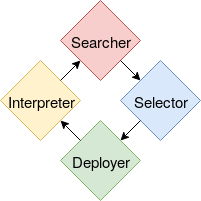
\includegraphics[scale=0.8]{Design}
\end{figure}
\section{Implementation}
How the implementation was done and tested, with
particular focus on important / novel algorithms and/or
data structures, unusual implementation decisions, novel
user interface features, etc.
\section{Evaluation and Critical Appraisal}
You should evaluate your own work with respect to your
original objectives. You should also critically evaluate
your work with respect to related work done by others.
You should compare and contrast the project to similar
work in the public domain, for example as written about
in published papers, or as distributed in software available to you. 
\section{Conclusions}
You should summarise your project, emphasising your
key achievements and significant drawbacks to your
work, and discuss future directions your work could be
taken in.
\newpage
\bibliographystyle{ieeetr}
\bibliography{Dissertation}
\newpage
\section*{Appendices}
\subsection*{Testing Summary}
\subsection*{User Manual}
\end{document}